% !TEX root = ../../thesis.tex
\chapter{Open diffusion} % (fold)


\section{Introduction} % (fold)



We will discuss several aspect concerning towards open science and diffusion.




\section{Poppy: an open science project}

For the moment, the Poppy project is actually an Inria project, led by the Flowers team. Yet the project potential is more universal and the fact it is owned by an entity reduces the scope of its applications and users, and therefore its societal impact.


Also, if we really want to transform the Poppy project into a real open science project, I think we should let go the project, I mean what the Poppy project should not anymore an Inria project, or a Flowers Team project nor a Matthieu Lapeyre's project. It should not be own by anyone because people will not be interested by participate in the success of someone project, it should be an anonymous project based on open science and education values.


For sure, we cannot just let the project by its own, maybe the best way to make this project independant would be to transfert it to an association with general assembly composed by members from several countries and universities



\section{Improving our impact in the open hardware community: Modularity} % (fold)

As we discussed longly in this thesis, Poppy has a modular morphology. This modularity is expressed with all technologies involved. For the mechanics, we use 3D printing techniques allowing to produce quick and low-cost parts. For the electronics, we designed a electronics board based on Arduino allowing to easily plug new sensors. Finally for the software, we built a library using an modular architecture both for the low-level thanks to I/O controllers and for the high-level with primitives paradigms.

As we saw in the chapter REF, this modularity allows for quick experimentation over morphological variants while the technology used are robust and easy-to-use.


\subsection{Modularity in the open source software} % (fold)

Open source software is very successful and widespread among the community of developers. Yet the first initiative

The Modularity refers to the manner in which a design is decomposed into different "modules". It is based on the notion of interdependence within modules and independence between modules~\cite{baldwin2000design}. This concept encompasses two related ideas: the need to allow work on a given module to be carried out without affecting other modules in the design, a concept known as "loose-coupling", and the need for well-designed "interfaces" between these modules~\cite{maccormack2006exploring}.

The concept of modularity appears as a fundamental property in the the open source software collaboration. Indeed, code modularity allows the overall project to be divided into much smaller and well-defined tasks that individuals can tackle independently from other tasks and without affecting other aspects of the program.

Thus Linus Torvalds, emphasized modularity as a design criterion early in the development of Linux~\cite{dibona1999open}. Indeed without modularity, it would be improbalbe that contributors could understand the whole design architecture to have a relevant contribution. It would be difficult to add new features or fix bug without affecting other part of the design. Linux needed to be modular to attract and facilitate a developer community. Code modularity allows partitioning of work among a global pool of developers and facilitates the recruitment of new contributors, as it reduces their learning curve to a subset of modules rather than the entire project~\cite{fitzgerald2004critical}.

\cite{lerner2002some}
A particular area of revision was the Application Program Interface (API), which allowed the development of Apache features to be very 'modular'. This step enabled programmers to make contributions to particular areas without affecting other aspects of the program



Moreover some insights show that the architecture of a product developed by a highly distributed team of developers is more modular than another product of similar size developed by a co-located team of developers~\cite{maccormack2006exploring}.




Thus, within a modular architecture, new module designs may be substituted for older ones easily and at low cost



Modularity is comming to the hardware (project Google)

\cite{narduzzo2008modularity} in GNU/Linux

\cite{lerner2002some}
A particular area of revision was the Application Program Interface (API), which allowed the development of Apache features to be very 'modular'. This step enabled programmers to make contributions to particular areas without affecting other aspects of the program

Various efforts by corporations selling proprietary software products to develop additional products through an open source approach have been undertaken.One of the most visible of these efforts was Netscape's 1998 decision to make 'Mozilla', a portion of its browser source code, freely available.This effort encountered severe difficulties in its first year, only receiving approximately two dozen postings by outside developers. Much of the problems appeared to stem from the insufficiently modular nature of the software: reflecting its origins as a proprietary commercial product,the different portions of the program were highly interdependent and interwoven

An interesting question is why corporations do not replicate the modular structure of open source software in commercial products more generally.One possibility may be that modular code,whatever its  virtues for a team of programmer working independently is not better for a team of and working together.




Another layer of modularity can be expressed at the technological level. Indeed, open source collaboration is much more effective and useful when technology are contain into module combined together rather than one big
The technological modularity allows a better impact in the open source community because people can extract one of the module to include it in their project.

If the stuff to hand isn't modular, you can't really share, because your stuff isn't compatible with other people's stuff. If it isn't modular, you can't share out tasks and scale. If you can't share out tasks, you can't have people working independently, at their own pace and in their own way, which means the project isn't really open. If it isn't modular, you can't swap in some new elements while leaving everything else untouched, which means no "release early, release often", no experimentation, no rapid evolution. Modularity is indispensable.


\section{Tools for hardware} % (fold)
\label{sec:tools_for_hardware}

Solidworks Eagle

% section tools_for_hardware (end)

\section{Production/Distribution: an alternative approach} % (fold)

\subsection{A research lab is not a Start-Up} % (fold)
Poppy includes three main parts: its mechatronic structure (skeleton and motors); its electronics; its software.

Reproducing and rebuilding the mechatronic structure is easy: the open-source skeleton can be printed on personal 3D printers (or using online services for higher quality printing), and motors are bought off-the-shelf (motors are currently not open-source, but very standard). Obtaining and using the software is very easy: just download on the Poppy web site.

But the fabrication of electronics is challenging. It is not yet possible to produce electronics components at home, and many institutional users do not have the competence or motivation to do so. There are some kickstarter projects going on a way to facilitate the process, yet they are not ready and won't be ready until a couple of years.

The current classical approach to build and distribute this electronics boards is to raise funding allowing the manufacturing of hundreds of boards which can then be sold by a distribution company. But a french research institute like Inria is not a distributor,  is not even legally allowed to do.

Furthermore, even if one could buy or build easily all components, some users (e.g. artists) might want to obtain and use an already fully assembled Poppy robot. Thus, a structure capable of building and distributing the electronics, as well as the mechatronics and/or the robot fully assembled is needed.

Yet, the mission of a research team at Inria is to do research, and find ways to apply and transfer the results of this research, but not directly to produce and sell a commercial product. If a commercial product can emerge from our research, one way to exploit it is to create a start-up company which will set up a business plan around it, probably based on a production in Asia and then a worldwide distribution to research laboratories, universities and fablabs (see Figure \ref{fig:classic})

\begin{figure}[h]
    \begin{center}
        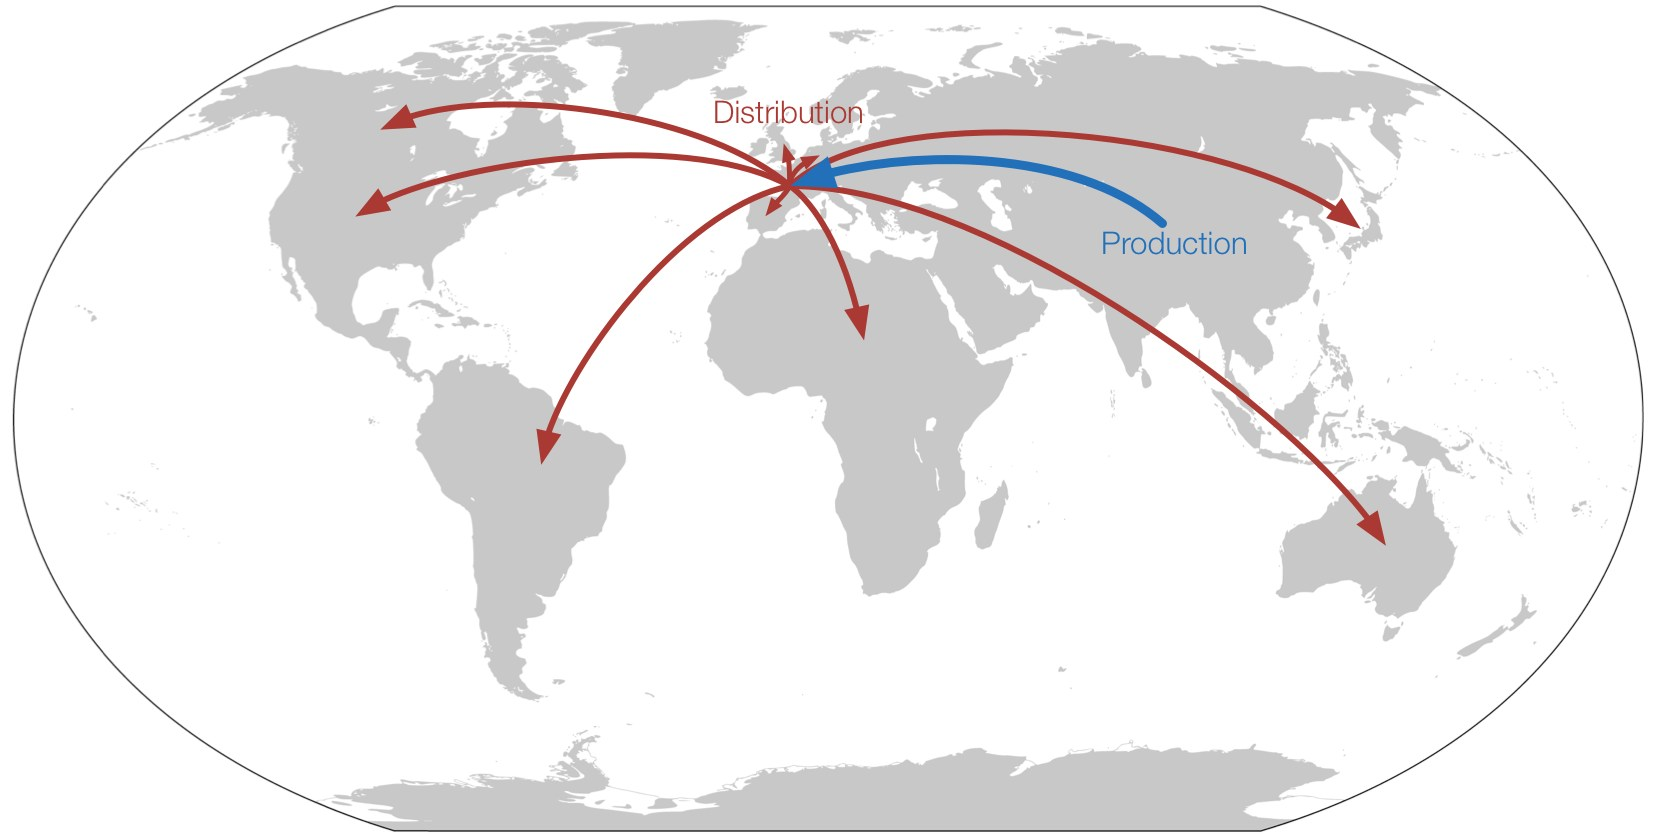
\includegraphics[width=14cm]{classic_production_distribution.jpg}
    \end{center}
    \caption{Classical approach for technology production and distribution}
    \label{fig:classic}
\end{figure}


But Poppy is not designed to be a standard commercial product. While it might foster the creation of an economical ecosystem and jobs, its main purpose is to become an educational tool that remains open, as well as rather low cost and easily reproducible. If the goal would have been to make it profitable, it would be necessary to sell it at a much higher price. The robot wouldn't be as accessible at it should to ensure the achievement of its scientific diffusion and educational missions... We would loose the intrinsic purpose of Poppy.

\section{Toward local open factories } % (fold)

Meanwhile, the "makers revolution" is gaining momentum~\cite{anderson2012makers} and more and more Fablabs are created around the world. As a main mission of Poppy is to be a educational platform, Poppy could become a popular platform used, hacked, transformed within the natural FabLab activities. But also, and this is the direction explored below,  it would make sense that Poppy, as a whole or subsets of its components, be produced and distributed by Fablabs, and thus becoming a tool used by Fab Lab to develop and robustify the economic ecosystem in which they live.

\subsection{Toward an alternative model} % (fold)

An original and constructive organizational process would be to take advantage of the production phase for educational purposes. In this context, each fablab would have the possibility to produce, assemble and sell Poppy to local actors (see Figure \ref{fig:world_fab}). Thus the production phase can become a training support for the use of 3D printing techniques and the manufacturing of electronic circuits, and later on be exploited through selling the constructed platforms.


\begin{figure}[tb]
    \begin{center}
        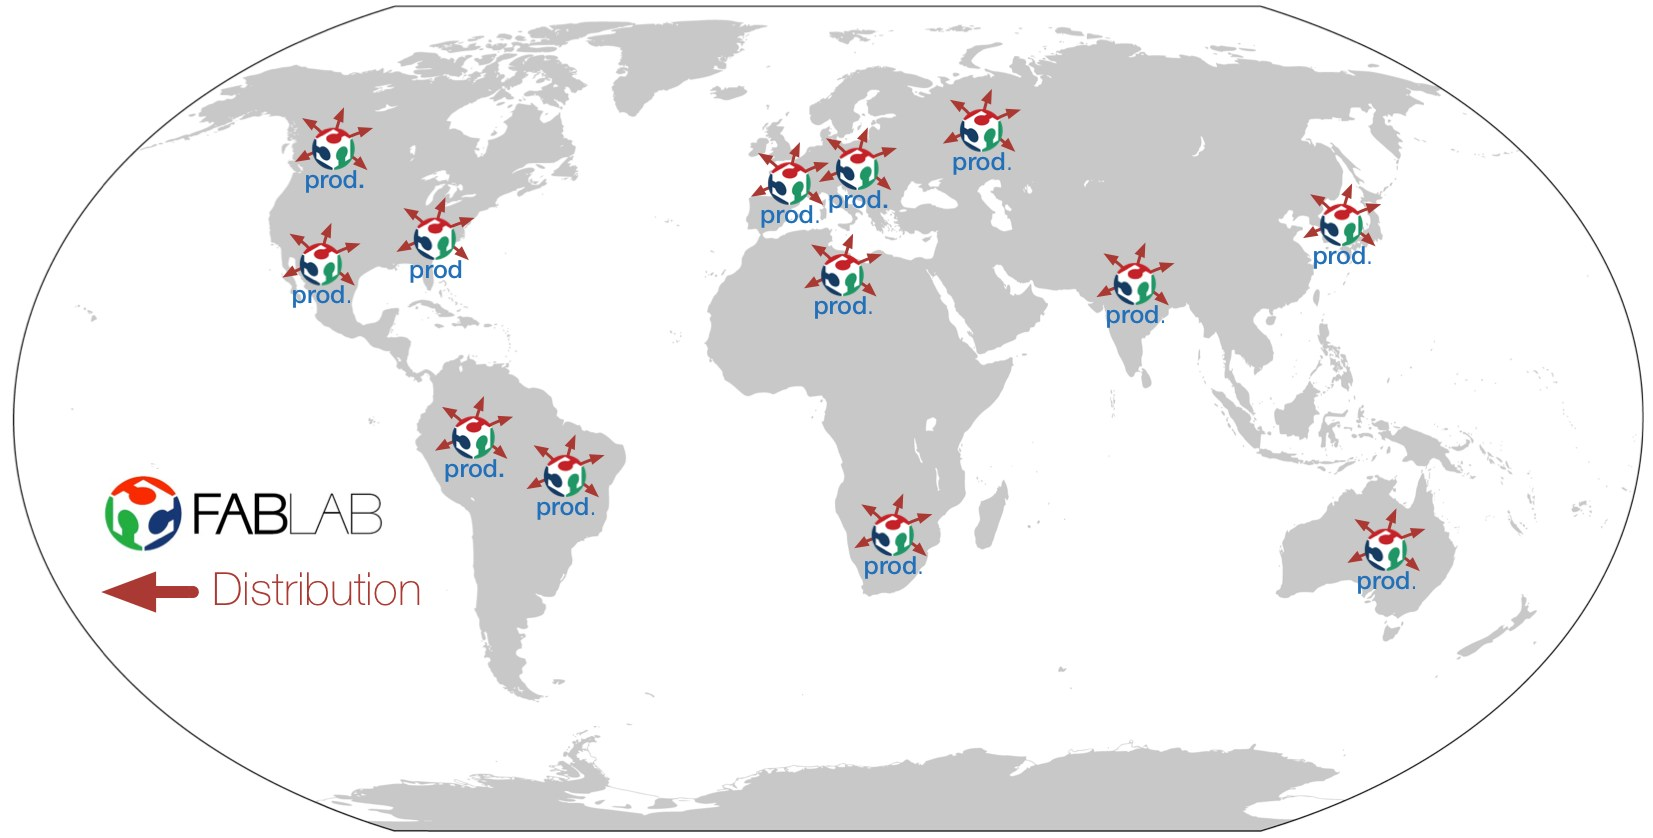
\includegraphics[width=14cm]{fabusine_distribution_world.jpg}
    \end{center}
    \caption{Fabrication and distribution locally done by Fablabs}
    \label{fig:world_fab}
\end{figure}


Also in a context where fablabs need to find an economic model, several sources of income may be found thanks to the distribution of platforms such as Poppy. The first and most obvious one is the sale to local actors of fully-assembled and functional Poppy robots produced by the Fablab. But a more advanced model can emerge. Poppy is a development robotic platform: it means that it can and will be broken, meaning that Fablabs may extend theirs commercial offers. Among them we can cite:

\begin{itemize}
    \item Ensure a support (repairs, upgrades, ...) and may sell maintenance contracts with labs/school/university and even other 3rd party FabLabs.
    \item Provide a customisation service to adapt Poppy to specific needs (e.g. a university or lycée that would like to have a Poppy on wheels rather than legs)
    \item For an event or artist residency: The FabLab could rent a robot and provide a technician,
    \item Propose profesional formation to 3D printing to companies
    \item ...
\end{itemize}

From these kinds of interaction, links and collaboration between local actors and Fablabs may emerge leading to other potentially funded projects.

\subsection{Promote local collaboration} % (fold)

Beyond the act of production and sales, Poppy could become a pretext to promote the linkage and exchange between local actors from multiple backgrounds. At the scale of a city or region, we can easily imagine a distribution of roles where several FabLabs could collaborate to build and distribute different parts of Poppy depending on their motivations, skills and equipements.
Also, it helps to connect the fablabs with local actors, public/private research labs, companies, schools/universities or artists (see Figure \ref{fig:local_synergy})

\begin{figure}[tb]
    \begin{center}
        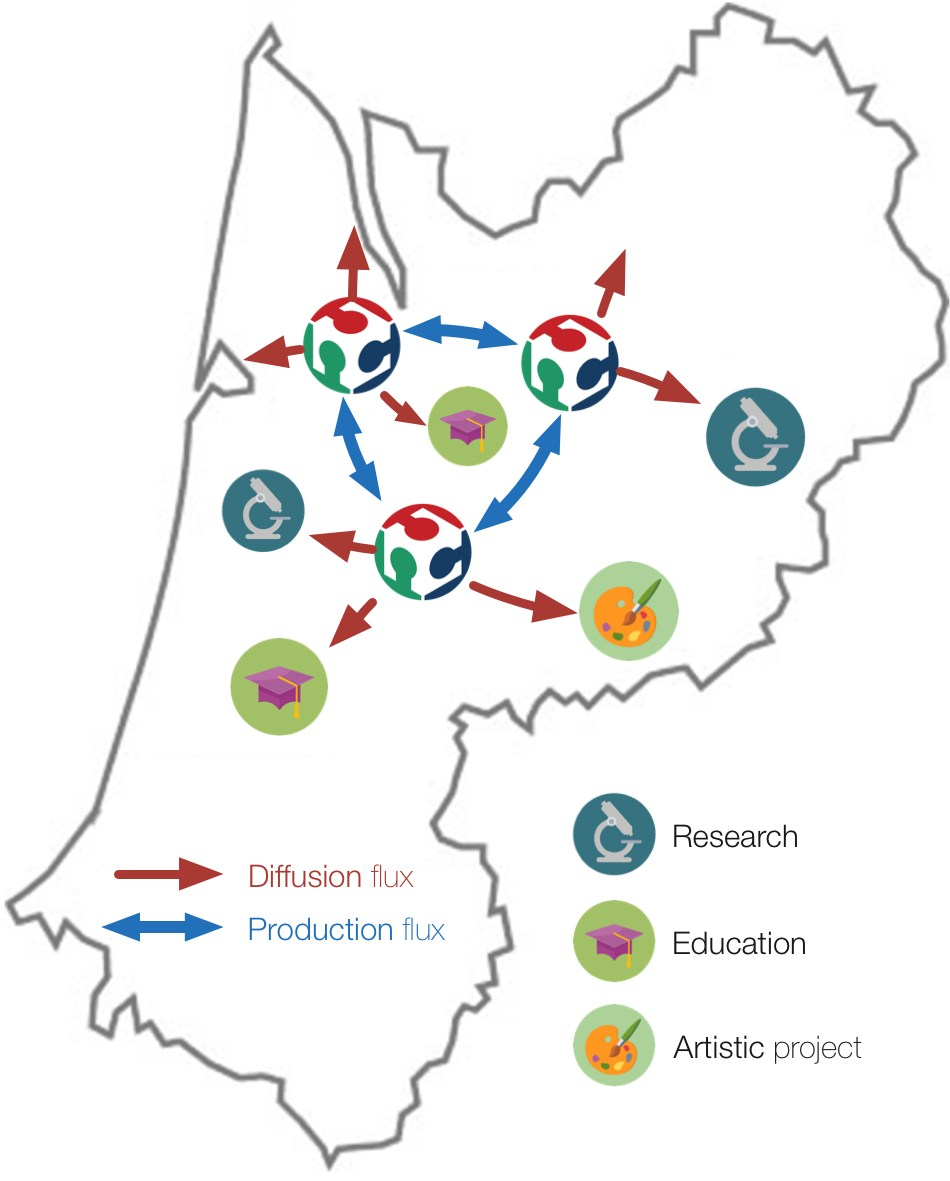
\includegraphics[height=10cm]{fabusine_local.jpg}
    \end{center}
    \caption{A synergy can emerge between Fablabs and local actors}
    \label{fig:local_synergy}
\end{figure}

\subsection{What is the role of the Flowers research team in such a process? } % (fold)

The Flowers research team's role remains essential. As the founders, designers and leaders of both the technological platform and its surrounding philosophy of openness and innovation, the Flowers team continues to improve the platform, take a central role in animating the community of users, and design new uses with scientists, educators, geeks and artists. Within this process, the Flowers team also coordinates the growing of the community of contributors and users, and designs strategies to ensure both the quality and sustainable development of the platform and its uses.

Among the tools used by the Flowers team to ensure such quality and sustainable development is through the control of the "Poppy" brand, and through policies/charters:

\begin{itemize}
\item The "Poppy" brand is owned by Inria, and the use of the brand by 3rd parties like FabLabs will only be possible through agreements ensuring that the Poppy project policies and philosophy is implemented;
\item Agreements take the form of charters/policies between Inria and FabLabs specifying guidelines to follow to ensure both quality and that each party (Inria, FabLab, users) finds its interest.
\end{itemize}

On the Inria side, the creation of an association which role would be to spin-off this technology development, community animation and quality control, is under consideration.


\subsection{conclusion} % (fold)
Poppy can be one of the first project launching this new kind of production and distribution process. The last months we met several of the main French FabLab. While their are quite enthousiast with this idea, the organisation is not completely ready to go on this way and we will certainly have to use the two ways to distribute Poppy. The first ones will be to let reseller create kit and sold them.







